\documentclass[a4paper,12pt]{article}
\usepackage{amsmath}
\usepackage{amssymb}
\usepackage{geometry}
\usepackage{listings}
\usepackage{xcolor}
\usepackage{graphicx}

\geometry{top=25mm, bottom=25mm, left=25mm, right=25mm}

\lstset{
  basicstyle=\ttfamily\footnotesize,
  breaklines=true,
  numbers=left,
  numberstyle=\tiny,
  keywordstyle=\color{blue},
  commentstyle=\color{green!50!black},
  stringstyle=\color{red!60!black},
  frame=single,
}

\title{地面と球の影の計算}
\author{}
\date{}

\begin{document}

\maketitle

\section*{概要}
本ドキュメントでは、光源と球の影が地面に投影されるシミュレーションをMATLABで実装する方法を示します。地面は離散的なデータとして与えられ、影の計算には光線追跡法と球の交差判定を使用します。影は地面のカラーデータとして表現されます。

\section*{理論的背景}
影の計算には次の2つの主要なステップがあります。

\subsection*{1. 光線のモデル}
光源 $L$ から球の表面上の任意の点 $P$ への光線を定義します。この光線のベクトルは以下の式で表されます。
\[
\mathbf{v} = \mathbf{P} - \mathbf{L}
\]
ここで、$\mathbf{P}$ は球上の点、$\mathbf{L}$ は光源の位置を表します。

\subsection*{2. 球と光線の交差判定}
光線 $\mathbf{v}$ が球と交差するかを判定するために、球の方程式を利用します。球の方程式は以下のように表されます。
\[
\|\mathbf{X} - \mathbf{C}\|^2 = R^2
\]
ここで、$\mathbf{C}$ は球の中心、$R$ は球の半径、$\mathbf{X}$ は球の任意の点を表します。

光線 $\mathbf{v}$ をパラメータ $t$ を用いて表すと、交差する点は以下の式で求められます。
\[
\mathbf{X}(t) = \mathbf{L} + t \mathbf{v}
\]
これを球の方程式に代入し、$t$ を解きます。結果は二次方程式の解として得られます。
\[
t = \frac{-b \pm \sqrt{b^2 - 4ac}}{2a}
\]
ここで、
\[
a = \|\mathbf{v}\|^2, \quad b = 2(\mathbf{L} - \mathbf{C}) \cdot \mathbf{v}, \quad c = \|\mathbf{L} - \mathbf{C}\|^2 - R^2
\]

\subsection*{3. 地面の色を変更}
影が落ちる位置を地面上で計算し、その位置の色データを黒(0)に変更します。これにより、地面のカラーデータを通じて影を可視化します。

\section*{MATLABコード}
以下はMATLABでの実装コードです。

\lstinputlisting[language=Matlab, caption=MATLABコード: 影の計算と可視化]{shadowSample_descreate_changeColor.m}

\section*{動作説明}
1. 地面のデータを離散的に定義します。地面は連続データから補間可能な形で提供されます。
2. 球の各頂点から光線をトレースし、影が地面上に落ちる点を計算します。
3. 球と光線の交差判定には二次方程式の解を利用します。
4. 地面の色データ(カラーデータ)を影の位置に基づいて変更し、影を可視化します。

\section*{結果例}
以下に影を可視化した結果例を示します。

\begin{figure}[h]
    \centering
    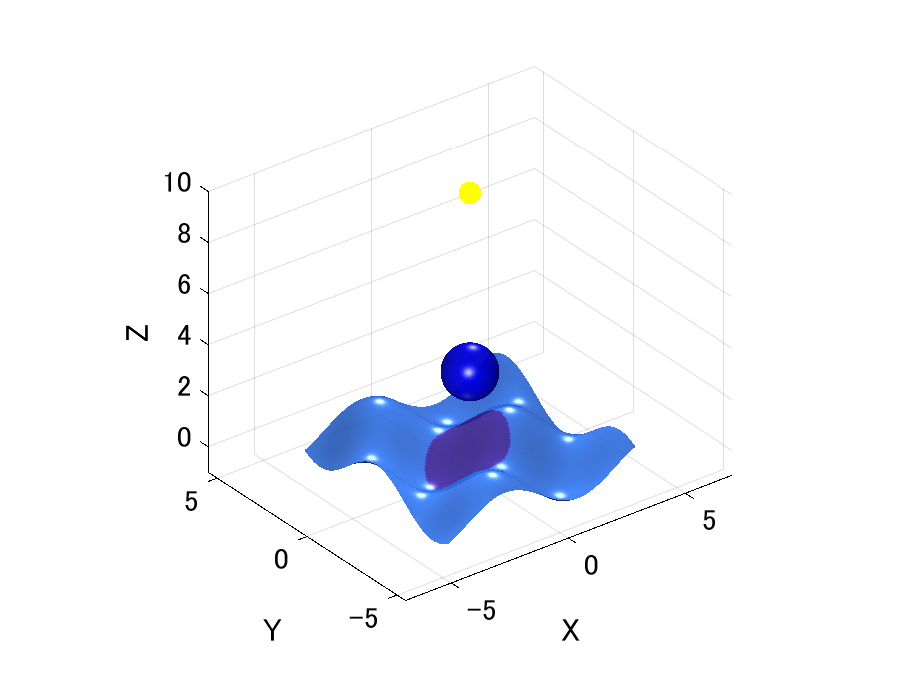
\includegraphics[width=0.8\textwidth]{shadow_example.eps}
    \caption{光源、地面、球、および影の可視化}
\end{figure}

\section*{まとめ}
本プログラムは、光源からの光線を利用して影を計算し、地面上の色を動的に変更することで影を可視化する方法を示しました。この手法は球以外の形状や複雑な地形にも応用可能です。

\end{document}
